\documentclass{ximera}

\usepackage{microtype}
\usepackage{tikz}
\usepackage{tkz-euclide}
\usetkzobj{all}
\tikzstyle geometryDiagrams=[ultra thick,color=blue!50!black]

\renewcommand{\epsilon}{\varepsilon}



\title{Spherical lunes and triangles}
\begin{document}
\begin{abstract}
In this activity we explore the areas of lunes and triangles on the sphere.
\end{abstract}
\maketitle



\section{Spherical lunes}

In the picture we have shaded in an `$\alpha$-lune' on the $R$-sphere in
euclidean $3$-space.%
\begin{image}
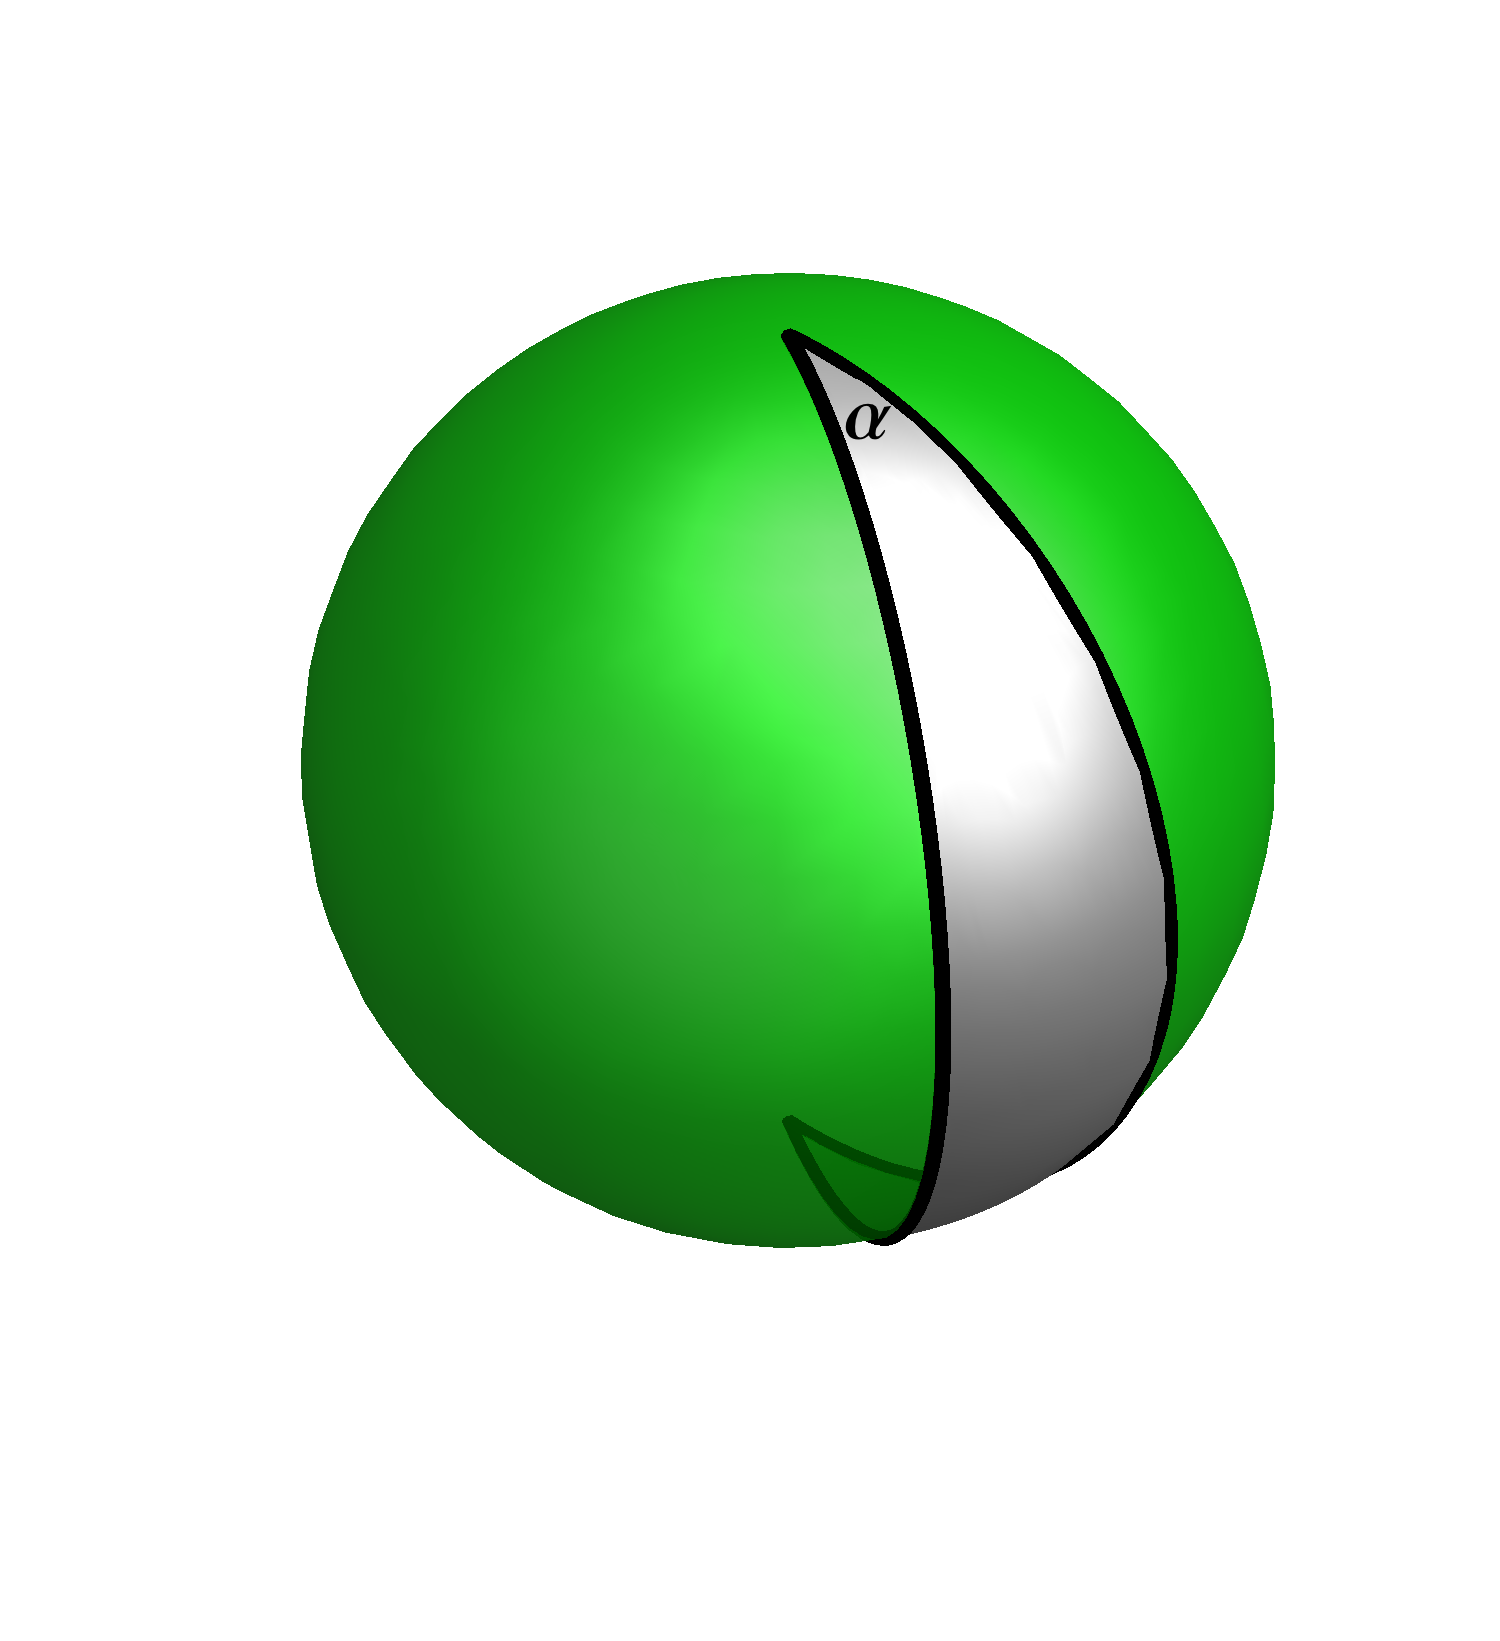
\includegraphics[width=3in]{W13_3.png}%
\end{image}


The lune has two vertices. They are at opposite (antipodal) points on the
$R$-sphere, that is, the line in euclidean $3$-space that joins the two
vertices runs through the center of the sphere. The angle at a vertex of the
lune is $\alpha$ radians.

\begin{problem}
\label{67} Explain why the area of the $\alpha$-lune is $2\alpha
\cdot R^{2}$.
\end{problem}


\section{Spherical triangles}

If a triangle on the sphere of radius $R$ has interior angles with radian
measures $\alpha$, $\beta$, and $\gamma$, it can be covered three times by
lunes as shown in the figure below.%
\begin{image}
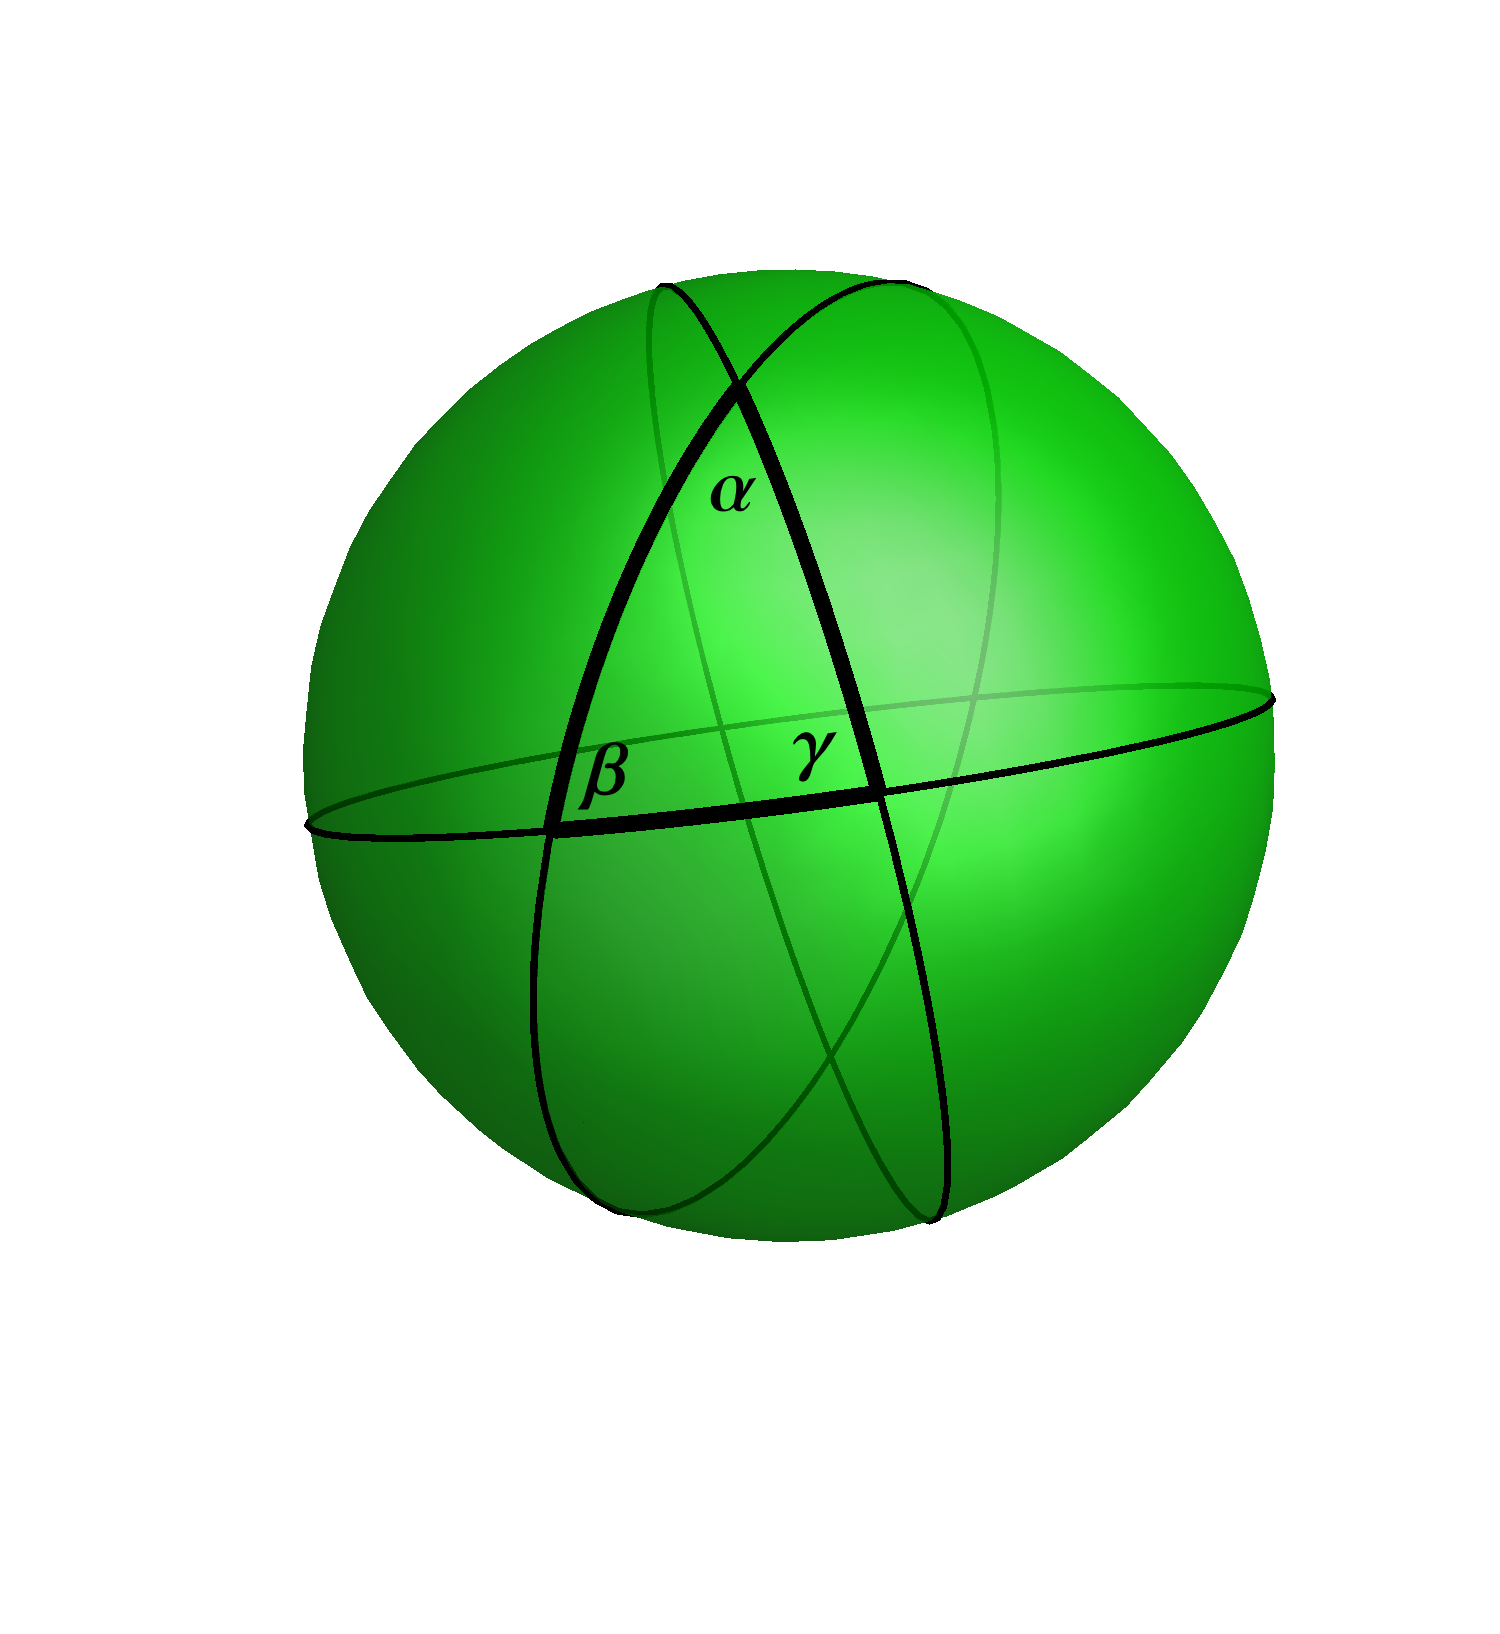
\includegraphics[width=3in]{W13_4.png}%
\end{image}
Notice that each lune has one vertex at a vertex of the triangle and angle
equal to that interior angle of the triangle. The other vertices of each lune
are vertices of an `opposite' triangle that has the same area as the given one
since it is just the image of the given one under the rigid motion%
\[
\left(  \underline{\hat{x}},\underline{\hat{y}},\underline{\hat{z}}\right)
=
\begin{bmatrix}
  \hat{x} & \hat{y} &\hat{z}
\end{bmatrix}  
\begin{bmatrix}
-1 & 0 & 0\\
0 & -1 & 0\\
0 & 0 & -1
\end{bmatrix}.
\]
The three lunes cover the triangle three times. The three opposite
lunes cover the opposite triangle three times. If you take all six
lunes together, they cover each of the two triangles three times and
everything else exactly once.

\begin{problem}
Show that the area of the spherical triangle is given by the
formula%
\[
R^{2}\left(  \left(  \alpha+\beta+\gamma\right)  -\pi\right).
\]
\begin{hint}
Use the previous problem.
\end{hint}
\end{problem}


\begin{problem}
Give a formula for the area of any spherical $n$-gon.
\begin{hint}
Divide the spherical $n$-gon into spherical triangles.
\end{hint}
\end{problem}


\begin{problem}
Summarize the results from this section. In particular, indicate which
results follow from the others.
\begin{freeResponse}
\end{freeResponse}
\end{problem}

\end{document}
